\Chapter{Pályageneráló algoritmusok}

Ebben a fejezetben három darab generálási módszert fogok bemutatni, amelyek a Perlin zaj, a celluláris automata, valamint a Random Walk algoritmusok. Mindhárom algoritmust a Unity keretrendszerben implementáltam és vizsgáltam meg, hogy melyik módszer illeszkedne legjobban a játékomhoz.

\Section{A térképgenerálás megtervezése}

Egy olyan dungeon-stílusú térképet szeretnék létrehozni, amelynek a külső szélei mindig falak, amelyek nem engedik leesni a játékost a pályáról, így a játék határai egyértelműen megmaradnak, valamint lehetővé teszi a játékosok számára, hogy szabadon navigáljanak anélkül, hogy áthatolhatatlan akadályokba ütköznének, például olyan falakba, amelyek megakadályozzák őket a tárgyak begyűjtésében. Tehát olyan pályageneráló algoritmus illeszkedne a játékomhoz, amely nem generál elzárt tereket, szobákat.

A térképgenerálás eredményeként a térkép egy logikai értékű mátrix:

\[
m_{ij} = 
\begin{cases} 
1, & \text{ha a cella} (i,j) \text{ teli,} \\
0, & \text{ha a cella} (i,j) \text{ üres}
\end{cases}
\]

Bináris érték használatával különböztetjük meg, hogy hova kerüljön a játékban fal jellegű elem. Az 1 bekapcsolva, a 0 pedig kikapcsolva jelzi ezt. Az összes térképünket egy 2D-s egész számtömbben tároljuk, amelyet minden egyes funkció végén (kivéve, amikor renderelünk) visszaküldünk a felhasználónak.\cite{mapgenerator}

Az új térkép generálása előtt a térképen a meglévő tile-ok törlődnek. Ez biztosítja, hogy az új térkép generálása üres vászonnal kezdődjön, megakadályozva az új adatok átfedését vagy összeolvadását a régi tile-okkal. Ezután egy metódus segítségével legenerálunk egy $N \times $N méretű tömböt, amiben az értékek a 0 vagy 1 értéket vehetik fel. Miután a tömb legenerálása befejeződött, meghívjuk a procedurális térképgeneráló algoritmusunkat, majd egy renderelő függvényt, amely az általunk kiválasztott tiletípust felfesti a térképre. A térképgenerálás folyamatábrája \aref{fig:generationflowchart}. ábrán megtekinthető.\cite{mapgenerator}

\begin{figure}[ht]
\centering
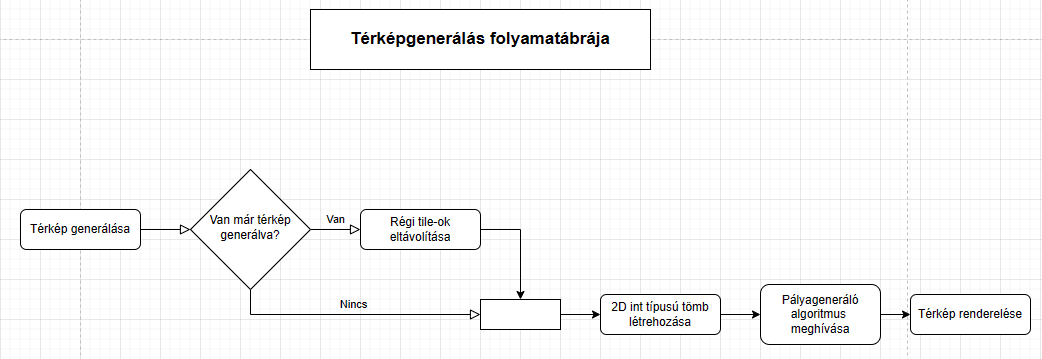
\includegraphics[width=\textwidth]{images/generationflowchart.png}
\caption{A térképgenerálás folyamatábrája}
\label{fig:generationflowchart}
\end{figure}

\Section{A térképgenerálás logikáját megvalósító algoritmusok bemutatása}

Ebben a fejezetben a térképek generálásáért felelős metódusokat fogom részletesen bemutatni. Ezek a metódusok a procedurális térképgenerálás alapvető keretét jelentik, ahol a \texttt{GenerateArray()} metódus létrehozza a térkép adatszerkezetét és kezdeti feltételeit, a \texttt{RenderMap()} metódus pedig az adatok játszható vagy látható formába való renderelésének mechanizmusaként szolgál. Ez a kétlépcsős folyamat -- az adatok létrehozása és az adatok renderelése -- központi szerepet játszik a játékom procedurális tartalomgenerálásában, lehetővé téve a térképek létrehozásának automatizálását.

\SubSection{A GenerateArray() metódus}

A \texttt{GenerateArray()} függvénynek a célja egy 2D-s \texttt{int[,]} típusú tömb létrehozása és inicializálása, amely a térképrácsot képviseli a procedurális generáláshoz. Ez a tömb szolgál alapként a procedurális mapgeneráló algoritmusok alkalmazásához a dungeon alaprajzának generálásához.

\textbf{Paraméterek:}
\begin{itemize}
\item \texttt{int width, int height} : Ezek a paraméterek határozzák meg a térkép méreteit, specifikusan a szélességét és a magasságát.
\item \texttt{bool empty} : Ez a logikai típusú változó határozza meg, hogy hogyan inicializáljuk a tömböt. Ha az értéke igaz, akkor üresként inicializáljuk, ha hamis, akkor pedig teliként.
\end{itemize}

Az \texttt{int[,] map = new int[width,height]} sorral egy új 2 dimenziós tömböt inicializálunk. A tömb minden eleme egy egész számot reprezentálhat.

A beágyazott \texttt{for} ciklusok a tömb minden egyes elemén végigmennek, az \texttt{x} a szélességen, az \texttt{y} pedig a magasságon iterál.

 A \texttt{map.GetUpperBound(0)} és a \texttt{map.GetUpperBound(1)} a tömb dimenzióinak felső határainak megadására szolgál. A \texttt{GetUpperBound(0)} az első dimenzió (szélesség) maximális indexét adja vissza, a \texttt{GetUpperBound(1)} pedig a második dimenzió (magasság) maximális indexét.

A \texttt{GetUpperBound} használata általában a tömb megadott dimenziójának utolsó érvényes indexét adja vissza. Egy szélesség és magasság dimenziójú tömb esetében a \texttt{GetUpperBound(0)} valójában a \texttt{width - 1}, a \texttt{GetUpperBound(1)} pedig a \texttt{height - 1} értéket adná vissza, mivel a tömbindexek 0-nál kezdődnek.

A belső cikluson belül az üres paraméter feltételes ellenőrzése dönti el, hogy a tömb helyét 0-val (ami üres vagy nyitott helyet jelez) vagy 1-gyel (ami kitöltött vagy blokkolt helyet jelez) töltse-e ki.

Miután a tömb teljesen feltöltődött, visszakerül a hívó számára. Ez a tömb most a kezdeti rácsállapotként szolgál a további feldolgozáshoz. Az alább látható metódus a \cite{mapgenerator} oldal alapján készült.

\begin{java}
public static int[,] GenerateArray(int width, 
    int height,bool empty)
{
    int[,] map = new int[width,height];
    for (int x = 0; x < map.
        GetUpperBound(0); x++)
    {
        for (int y = 0; y < map.
            GetUpperBound(1); y++)
        {
            if (empty)
            {
                map[x, y] = 0;
            }
            else
            {
                map[x,y] = 1;
            }
        }
    }
    return map;
}
\end{java}

\SubSection{A RenderMap() metódus}

A \texttt{RenderMap()} függvény felelős a generált térkép vizuális megjelenítéséért egy Unity \texttt{Tilemap}-en egy adott \texttt{TileBase} segítségével. Ez a függvény a numerikus térképadatokat (egy 2D-s egész számtömbben tárolva) a játéktérképen lévő tényleges tile-okká alakítja át.

\textbf{Paraméterek:}
\begin{itemize}
\item \texttt{int[,] map}: Egy két dimenziós tömb, amely a dungeon alaprajzát reprezentálja, ahol az egyes cellák értéke határozza meg, hogy üres vagy tele van-e az adott cella.
\item \texttt{Tilemap tilemap}: Ez a Unity \texttt{Tilemap}, amelyre a tile-ok fognak felrajzolódni.
\item \texttt{TileBase tile}: Ez a térkép kitöltött területeinek vizuális ábrázolására szolgáló tile (esetemben \texttt{RuleTile}).
\end{itemize}

A \texttt{tilemap.ClearAllTiles()} paranccsal, mielőtt az új térképet lerenderelnénk, töröljük az összes meglévő tile-t a térképről. Ez kulcsfontosságú annak biztosítása érdekében, hogy a korábbi tile-ok ne maradjanak láthatóak. Ez a metódus is egymásba ágyazott \texttt{for} ciklusokat használ ahhoz, hogy bejárja a map tömb minden elemét. 

A cikluson belül a függvény minden egyes koordinátánál (x, y) ellenőrzi az értéket. Az \texttt{if(map[x, y] == 1)} feltétel ellenőrzi, hogy az aktuális koordinátáknál lévő cella tele van-e (1 az érték). Ha tele van, akkor a \texttt{Tilemap} megfelelő pozíciójára egy új tile kerül. A \texttt{tilemap.SetTile(new Vector3Int(x, y, 0), tile)} parancs egy tile-t helyez el a \texttt{Tilemap (x, y)} pozíciójában. Az alább látható metódus a \cite{mapgenerator} oldal alapján készült.

\begin{java}
public static void RenderMap(int[,] map, 
    Tilemap tilemap, TileBase tile)
{
    //We clear the map to make
    //sure we don't overlap
    tilemap.ClearAllTiles();

    for (int x = 0; x < 
        map.GetUpperBound(0); x++)
    {
        for (int y = 0; y < 
            map.GetUpperBound(1); y++)
        {
            //1 = tile, 0 = no tile
            if (map[x,y] == 1)
            {
                tilemap.SetTile(new Vector3Int
                    (x, y,0),tile);
            }
        }
    }
}
\end{java}

\Section{A Perlin zaj}

A Perlin-zaj egy algoritmus, amelyet Ken Perlin hozott létre az 1980-as évek elején, és széles körben használják a játékfejlesztésben bármilyen hullámszerű anyag vagy textúra létrehozásához. Például a Perlin-zajt használhatjuk procedurális domborzati alakzatok (Minecraft szerű domborzati térkép hozható létre a Perlin-zaj algoritmus segítségével), tűzeffektek, víz és felhők létrehozásához. Ezek a hatások főleg a második és harmadik dimenzióban tükrözik a Perlin-zajt, de kiterjeszhető a negyedik dimenzióra is. Ezen kívül az algoritmus használható még az 1 dimenziós térben is, mint például egy „side-scroller” terep létrehozásához, vagy kézzel írt vonalak illúziójának megteremtésére. \cite{perlin2}

Sőt mi több, ha az algoritmust a 2. vagy a 3. dimenzióra is kiterjesztjük, valamint az extra dimenziókra úgy tekintünk, mint az időre, akkor meg is tudjuk a kreált alakzatokat animálni. Az \aref{tab:perlinnoise}. táblázatban néhány képet láthatunk a különböző méretű zajokról és néhány felhasználási módjukról futás közben. \cite{perlin1}

\begin{table}[ht]
\centering
\caption{A Perlin zaj felhasználási módjai}
\label{tab:perlinnoise}
\begin{tabular}{|c|c|c|}
\hline
Zaj dimenziószáma & A nyers zaj (szürkeárnyalatos) & Felhasználási mód \\
\hline
1 & 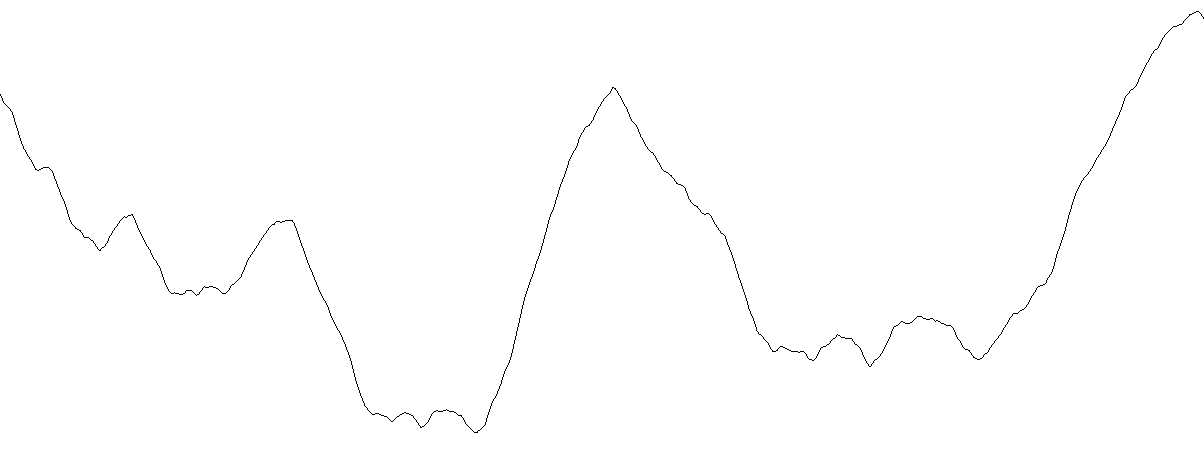
\includegraphics[width = 0.23\linewidth]{images/1dperlin.png} & 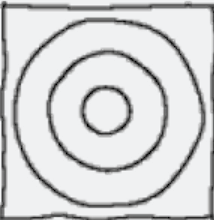
\includegraphics[width = 0.23\linewidth]{images/1dperlinusecase.png} \\
\hline
2 & 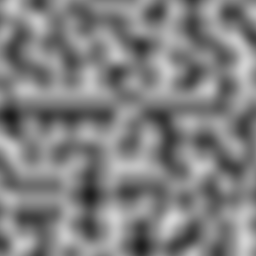
\includegraphics[width = 0.23\linewidth]{images/2dperlin.png} & 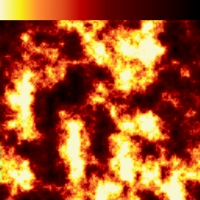
\includegraphics[width = 0.23\linewidth]{images/2dperlinusecase.png} \\
\hline
3 & 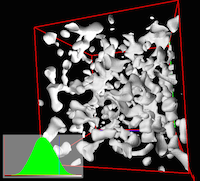
\includegraphics[width = 0.23\linewidth]{images/3dperlin.png} & 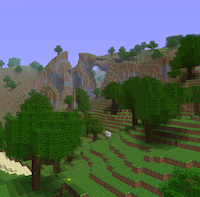
\includegraphics[width = 0.23\linewidth]{images/3dperlinusecase.png} \\
\hline
\end{tabular}
\end{table}

\newpage
A táblázatban lévő képeket a \url{https://adrianb.io/2014/08/09/perlinnoise.html} oldalról használtam fel.

A Perlin-zaj gradiens zajgenerálási technikát alkalmaz, ami a pontok közötti természetesebb és simább átmenetet eredményez. Ez a megközelítés élethűbbnek tűnő tájképet hoz létre. Az algoritmus egy rácshálós keretrendszerben működik, ahol a rácsháló minden egyes metszéspontjához egy gradiensvektor tartozik. Ezek a vektorok döntő fontosságúak a zaj mintázatának és irányítottságának kialakításában.

A Perlin-zaj egyik fő jellemzője a rácspontok közötti interpoláció alkalmazása, ami hozzájárul a jellegzetes simasághoz. Ez a sima átmenet éles ellentétben áll a teljesen véletlenszerű zajgenerálásra jellemző hirtelen változásokkal. A Perlin-zajt eredetileg 3D-s grafikához fejlesztették ki, de a 2D-s alkalmazásokban is széles körben használják, többek között a videojátékok terepgenerálásában és a procedurális textúrák létrehozásában.
A generált minták összetettségének fokozása érdekében az algoritmus gyakran alkalmaz rétegezési technikát, amely több "oktávnyi" zajt tartalmaz. Minden egyes oktáv külön frekvenciával és amplitúdóval működik, és amikor ezeket a rétegeket kombinálják, bonyolultabb és változatosabb mintákat hoznak létre. Az algoritmus állítható paramétereket kínál, mint például a frekvencia, az amplitúdó és a perzisztencia, ami lehetővé teszi a generált zaj megjelenésének részletes szabályozását, és a terep vagy a textúra testre szabott szimulációját.

A játékokban és a számítógépes grafikában való alkalmazásán túl a Perlin-zaj elterjedt más területeken is, mint például tudományos szimulációk készítése, ahol olyan természeti jelenségeket modellez, mint a felhőképződmények, vagy egy táj jellegzetességei.

\SubSection{A Perlin-zaj algoritmus implementálása és vizsgálata}

A \texttt{PerlinNoiseDungeon()} metódus a Perlin-zaj segítségével módosítja a rácsos térképet, hogy simább átmeneteket hozzon létre a kitöltött és üres terek között.

\textbf{Paraméterek:}
\begin{itemize}
\item \texttt{int[,] map}: A módosítandó kezdeti térképtömb.
\item \texttt{float modifier}: Egy skálázási tényező, amely a Perlin zajfüggvény frekvenciáját állítja be. Az értéke 0 és 1 között van.
\end{itemize}

A metódusban a Perlin-zajt a térképrács minden egyes koordinátájára úgy alkalmazzuk, hogy a koordinátákat megszorozzuk a modifier változóval. Ez a modifier változó befolyásolja a zaj "zoom" szintjét -- a magasabb értékek kisebb térrészeken belüli gyakoribb változást eredményeznek, ami töredezettebb mintázatot hoz létre, míg az alacsonyabb értékek szélesebb, simább átmeneteket eredményeznek.

Az egyes cellák zajértékének kiszámítása után a zajáértéket egész számra kerekítjük (0 vagy 1), hogy eldöntsük, hogy a cella fal vagy üres tér legyen.

A metódus a térkép határait kifejezetten falaknak állítja be a meghatározott élek fenntartása érdekében.

A függvény visszaadja a módosított térképtömböt az új terepjellemzőkkel együtt, készen állva a renderelésre. Az alább látható metódus a \cite{mapgenerator} oldal alapján készült.

\begin{java}
public static int[,] PerlinNoiseDungeon(
    int[,] map, float modifier)
{
    int newPoint;
    for (int x = 0; x < 
        map.GetUpperBound(0); x++)
    {
        for (int y = 0; y < 
            map.GetUpperBound(1); y++)
        {

            if ((x == 0 || y == 0 || 
                x == map.GetUpperBound(0) - 1 || 
                y == map.GetUpperBound(1) - 1))
            {
                //Keep the edges as walls
                map[x, y] = 1;
            }
            else
            {
                //Generate a new point using perlin noise,
                //then round it to a value of either 0 or 1
                newPoint = Mathf.RoundToInt(
                    Mathf.PerlinNoise(x * modifier, 
                    y * modifier));
                map[x, y] = newPoint;
            }
        }
    }
    return map;
}
\end{java}

A továbbiakban a Perlin-zaj által generált térképek vizsgálatáról lesz szó.

Mindegyik generált térkép $100 \times $100-as mátrixnak felel meg, amelyet 1-esekkel töltünk fel. A \texttt{modifier} változó értékét fogom növelni a vizsgálat során, az első érték a 0.05, a második a 0.10 és ez egészen a 0.30 értékig fog növekedni. A generált térképek \aref{fig:lowmodifyperlin}. ábrán és \aref{fig:highmodifyperlin}. ábrán láthatóak.

\begin{figure}[ht]
\centering
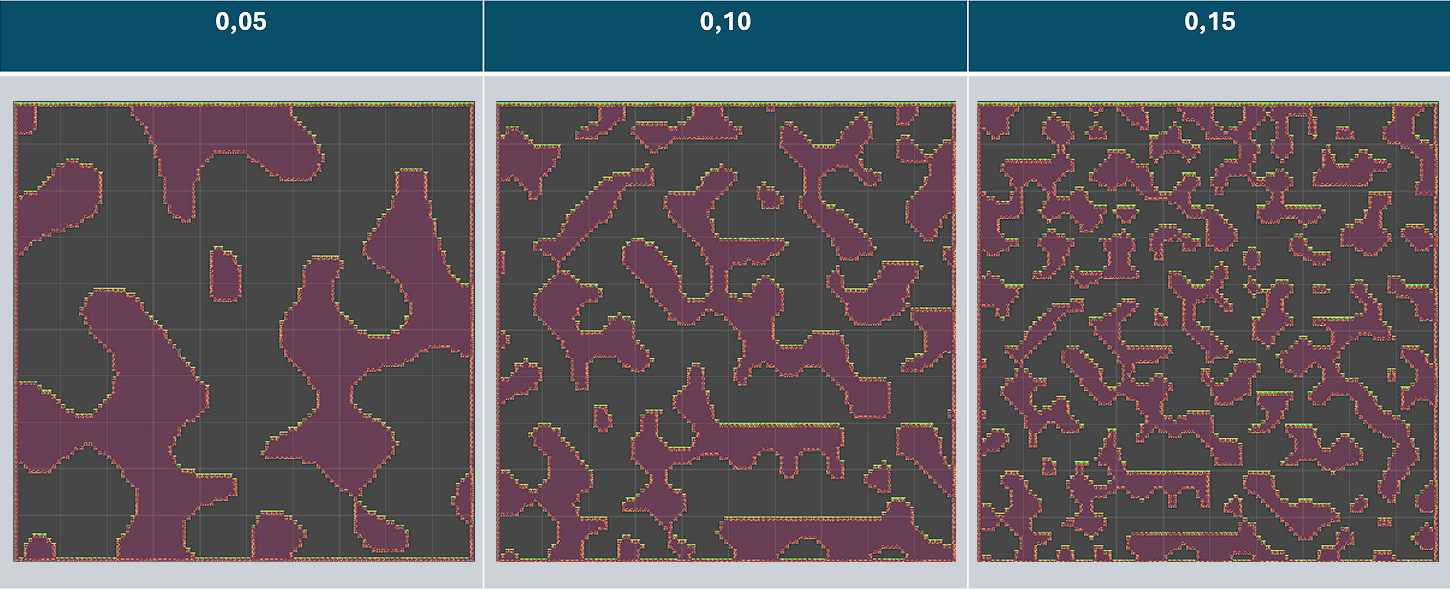
\includegraphics[width=\textwidth]{images/lowmodifierperlin.png}
\caption{ A \texttt{PerlinNoiseDungeon()} metódussal generált térképek 0.05, 0.10 és 0.15 \texttt{modifier} értékekkel}
\label{fig:lowmodifyperlin}
\end{figure}

\begin{figure}[ht]
\centering
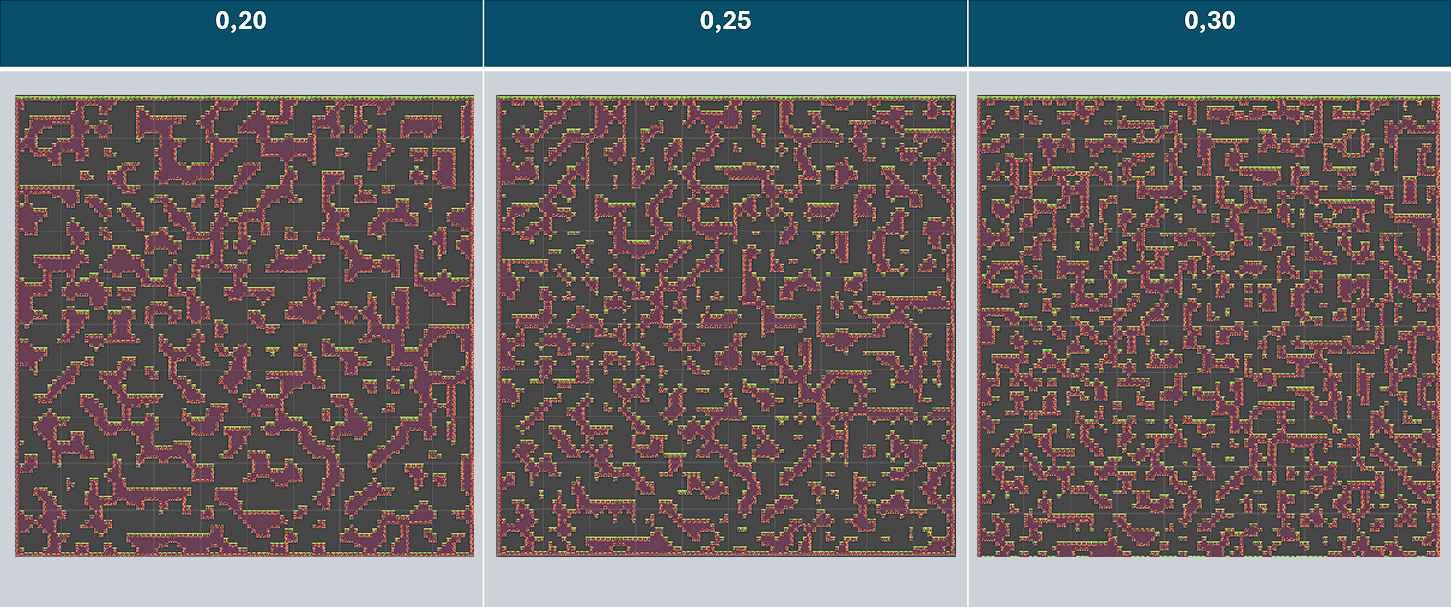
\includegraphics[width=\textwidth]{images/highmodifierperlin.png}
\caption{ A \texttt{PerlinNoiseDungeon()} metódussal generált térképek 0.20, 0.25 és 0.30 \texttt{modifier} értékekkel}
\label{fig:highmodifyperlin}
\end{figure}


Ahogy a generált térképeken is láthatjuk, az alacsonyabb modifier értékek általában nagyobb, összefüggőbb régiókat eredményeznek, amelyek szélesebb földtani jellemzőket, például széles barlangokat vagy nagy nyílt területeket szimulálnak. A magasabb módosító értékek széttöredezettebb és kuszább tereket hoznak létre, amelyek bonyolult alagútrendszereket vagy sűrű barlanghálózatot eredményeznek.

Ezek a különbségek úgy befolyásolhatják a játékmenetet, hogy a nagyobb, nyílt területek megkönnyíthetik a navigációt, könnyedebben teljesíthetőek lesznek a pályák, míg a bonyolultabb, magasabb modifier értékkel generált pályák nagyobb kihívást jelentőek lesznek, hosszabb játékidőt és frusztrációt eredményezhetnek.

Ezek a legenerált pályák nem feleltek meg az általam elvárt kinézetnek, mivel tartalmaznak olyan elzárt részeket, amelybe a játékos nem tud bemenni. Olyan játékoknál alkalmaznám ezt a fajta pályagenerálást, amelyeknél implementálva van az, hogy a játékos eltüntetheti, széttörheti a blokkot, mondjuk egy csákánnyal, vagy bombával.

\Section{A celluláris automata}

A celluláris automata, egy rácsalapú rendszerben működő számítási modell, amely egyszerűségében és összetettségében egyaránt lenyűgöző. Minden egyes sejt ezen a rácshálózaton két állapotban létezhet, amelyek az "él" vagy a "halott" állapotok. E sejtek fejlődését egyik generációról a másikra egy szabályrendszer határozza meg, amely jellemzően a szomszédos sejtek állapotán alapul. Ez a felállás, bár összetevőit és szabályait tekintve egyszerű, az azonos szabályokat követő sejtek együttes kölcsönhatása révén rendkívül bonyolult mintázatokat képes létrehozni. \cite{cellular}

A celluláris automaták egyik legismertebb példája Conway „Game of Life” című műve. Ez egy kiváló példa arra, hogy az alapvető szabályok hogyan eredményezhetnek összetett viselkedést, annak ellenére, hogy ez egy „zero-player” játék, ami azt jelenti, hogy a fejlődését a kezdeti állapota határozza meg, és nincs szüksége emberi játékostól származó cselekedetre, inputra. Az ember úgy lép kapcsolatba a játékkal, hogy létrehoz egy kezdeti konfigurációt, és megfigyeli, hogy hogyan fejlődik. A celluláris automata, valamint a „Game of Life” játék négy szabálya a következő: \cite{conway}
\begin{enumerate}
\item Minden olyan élő sejt, amelynek kettőnél kevesebb szomszédja van, „meghal” (ezt nevezzük alulnépesedésnek vagy veszélyeztetettségnek).
\item Minden olyan élő sejt, amelynek háromnál több szomszédja van, „meghal” (ezt nevezik túlnépesedésnek vagy túlzsúfoltságnak).
\item Minden élő sejt, amelynek két vagy három élő szomszédja van, változatlanul tovább él a következő generációig.
\item Minden halott sejt, amelynek pontosan három élő szomszédja van, életre kel.
\end{enumerate}

A kezdeti minta képezi a rendszer "magját". Az első generáció úgy jön létre, hogy a fenti szabályokat egyszerre alkalmazzák a mag minden sejtjére - a születések és halálozások egyszerre történnek, és azt a diszkrét pillanatot, amikor ez megtörténik, néha ticknek nevezik. (Más szóval, minden egyes generáció az előző generáció színtiszta függvénye.) A szabályok ismételt alkalmazása további generációk létrehozásához folytatódik. \cite{conway} A celluláris automata szabályait \aref{fig:cellularprincipals}. ábrán láthatjuk.

\begin{figure}[ht]
\centering
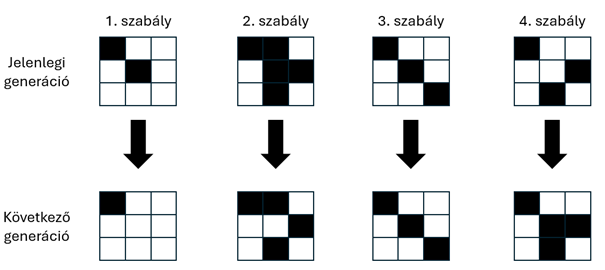
\includegraphics[width = \textwidth]{images/cellularprincipals.png}
\caption{A celluláris automata szabályai szemléltetve}
\label{fig:cellularprincipals}
\end{figure}

\newpage
A celluláris automata rugalmassága a testreszabhatóságban rejlik. A fejlesztők a szabályokat és az állapotokat az egyedi igényekhez igazíthatják, befolyásolva olyan szempontokat, mint a térkép sűrűsége és az útvonalak összekapcsolhatósága. A véletlenszerűség beépítésének képessége ellenére az automata determinisztikus jellege biztosítja az azonos kezdeti feltételekből származó konzisztens eredményeket, ami különösen hasznos a reprodukálható szintek létrehozásához. \cite{cellular}

A celluláris automata nem csak a szintek strukturálásában segít, hanem a vizuális látványt is fokozza, olyan mintákat generálva, amelyek esztétikailag szépek és a játékmenet szempontjából is praktikusak. Ezzel a tulajdonságával hatékony eszközzé válik a fejlesztők számára, akik dinamikus és megnyerő környezetet kívánnak létrehozni a 2D platformer játékokban, és az egyedi, változatos szintek létrehozásával jelentősen növeli a játék újra játszásának az esélyét. \cite{cellular}

\SubSection{A celluláris automata algoritmus implementálása és vizsgálata}

Ahhoz, hogy a \texttt{VonNeumannCellularAutomata()} metódus létrehozza a randomizált térképünket, először egy módosított térképet kell kreálnunk. A módosítás pedig nem más, mint a randomizáció.

A \texttt{ModifiedMapForCellularAutomata()} metódus megteremti egy celluláris automata folyamat előfeltételeit egy véletlenszerű kezdeti feltételeket tartalmazó térkép létrehozásával, amely aztán a következő lépésekben a von Neumann celluláris automata szabályaival lesz fejlesztve. Funkcionalitását tekintve ugyan azt csinálja, mint a \texttt{GenerateArray()} metódus, de miközben inicializálja a térképtömböt, nem egyenletesen tölti ki a térképteret, hanem randomizálva. Minden belső cellához véletlenszerű állapotot rendel (0 vagy 1) a \texttt{fillPercent} által meghatározott valószínűség alapján. Az alább látható metódus a \cite{mapgenerator} oldal alapján készült.

\begin{java}
 public static int[,] ModifiedMapForCellularAutomata(
    int width,int height, float seed, int fillPercent)
{
    //Seed our random number generator
    System.Random rand = new System.Random(
        seed.GetHashCode());

    int[,] map = new int[width, height];

    for (int x = 0; x < 
        map.GetUpperBound(0); x++)
    {
        for (int y = 0; y < map.GetUpperBound(1); y++)
        {
            if ((x == 0 || x == map.GetUpperBound(0) - 1 || 
                y == 0 || y == map.GetUpperBound(1) - 1))
            {
                //Ensure the walls on the sides of the map
                map[x, y] = 1;
            }
            else
            {
                //Randomly generate the grid
                map[x, y] = (rand.Next(0, 100) < 
                    fillPercent) ? 1 : 0;
            }
        }
    }
    return map;
}
\end{java}

A \texttt{VonNeumannCellularAutomata()} metódus a von Neumann szomszédságon alapuló celluláris automata technikát használja a generált térkép fejlesztésére.

\textbf{Paraméterek}
\begin{itemize}
\item \texttt{int[,] map} : Ez az a térkép, amelyet a függvény módosítani fog.
\item \texttt{int smoothCount}: Az iterációk (vagy generációk) száma, amelyeken a celluláris automata folyamat keresztülmegy.
\end{itemize}

A térkép többszörös átmeneteken megy keresztül a cellák állapotának fejlesztése érdekében. A több ismétlés jellemzően simább és összefüggőbb struktúrákat eredményez.

Csak a közvetlen szomszédokat (felfelé, lefelé, balra, jobbra) veszi figyelembe az egyes cellák evolúciója, ami leegyszerűsíti az interakciókat, és inkább az utak vagy nyitott területek létrehozására összpontosít, mint a komplex mintázatokra.

\textbf{Cellaállapot-frissítési szabályok}
\begin{itemize}
\item Kitöltött cella: Ha egy cellának több mint 2 környező kitöltött cellája van, akkor maga is kitöltött cellává válik.
\item Üres cella: Ha egy cellának 2-nél kevesebb kitöltött cellája van, akkor üres lesz.
\item Nincs változás: Ha egy cellának pontosan 2 szomszédja van, az állapota változatlan marad. Ez a szabály stabilitást biztosít a struktúrának, fenntartva a jelenlegi komplexitást.
\end{itemize}

A megadott számú iteráció elvégzése után a függvény visszaadja a továbbfejlesztett mapot, amely tükrözi a celluláris automata által végrehajtott változásokat. Az alább látható metódus a \cite{mapgenerator} oldal alapján készült.

\begin{java}
public static int[,] VonNeumannCellularAutomata(
    int[,] map, int smoothCount)
{
    for (int i = 0; i < smoothCount; i++)
    {
        for (int x = 0; x < 
            map.GetUpperBound(0); x++)
        {
            for (int y = 0; y < 
                map.GetUpperBound(1); y++)
            {
                //Get the surrounding tiles
                int surroundingTiles = 
                    GetVNSurroundingTiles(map, x, y);

                if ((x == 0 || 
                    x == map.GetUpperBound(0) - 1 || 
                    y == 0 || y == map.GetUpperBound(1)))
                {
                    //Keep our edges as walls
                    map[x, y] = 1; 
                }
                //von Neuemann Neighbourhood requires
                //only 3 or more surrounding tiles
                //to be changed to a tile
                else if (surroundingTiles > 2)
                {
                    map[x, y] = 1;
                }
                //If we have less than 2 neighbours,
                //set the tile to be inactive
                else if (surroundingTiles < 2)
                {
                    map[x, y] = 0;
                }
                //Do nothing if we have 2 neighbours
            }
        }
    }
    return map;
}
\end{java}

A fenti metódusban használt \texttt{GetVNSurroundingTiles()} metódus \cite{mapgenerator} célja a környező "kitöltött" cellák számának kiszámítása a von Neumann szomszédság alapján, amely csak a négy szomszédos cellát veszi figyelembe a fő irányokban: felette, alatta, balra és jobbra. A von Neumann szomszédságot reprezentáló ábra \aref{fig:vonNeumann}. ábrán látható.

\begin{figure}[ht]
\centering
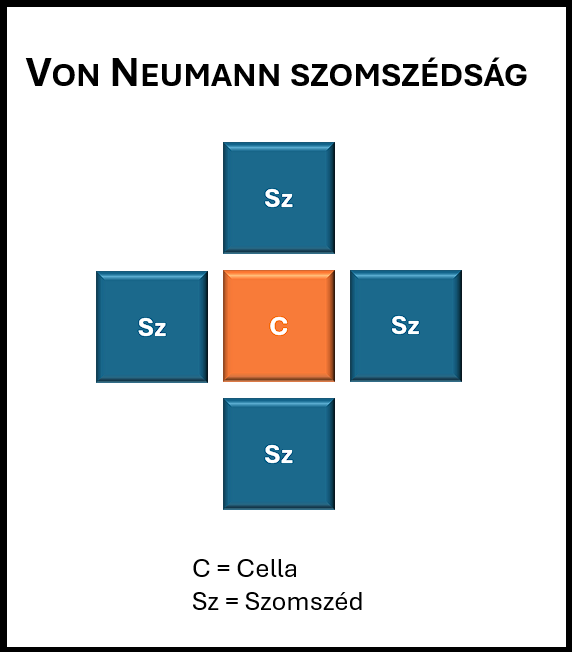
\includegraphics[scale = 0.4]{images/vonNeumann.png}
\caption{A von Neumann szomszédság}
\label{fig:vonNeumann}
\end{figure}

A továbbiakban a celluláris automata által generált térképek vizsgálatáról lesz szó.

Mindegyik generált térkép $100 \times $100-as mátrixnak felel meg, amelyet véletlenszerűen töltünk fel 1-esekkel és 0-ákkal. Először a \texttt{requiredFillPercent} változó fixálásával és a \texttt{smoothIterations} változó növelésével fogom vizsgálni a legenerált térképeket, majd a \texttt{smoothIterations} változó értékét fixálom és a \texttt{requiredFillPercent} értékét fogom növelni. A generált térképek \aref{fig:fixedPercentCellular}. ábrán láthatóak.

\begin{figure}[ht]
\centering
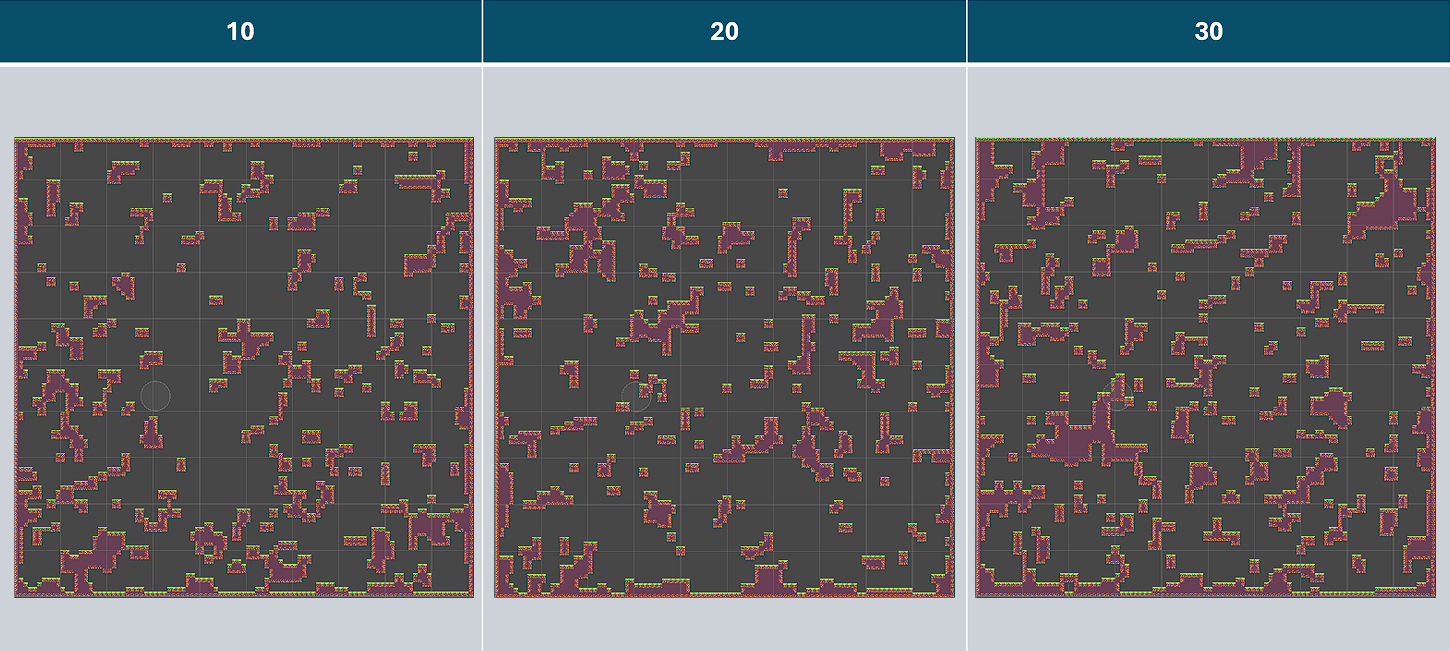
\includegraphics[width=\textwidth]{images/fixedpercentcellular.png}
\caption{Fixált \texttt{requiredFloorPercent} értékkel és változó \texttt{smoothIterations} értékkel generált térképek}
\label{fig:fixedPercentCellular}
\end{figure}

A fentebb látható legenerált térképeknél a \texttt{requiredFloorPercent} értéke fixen 40, a \texttt{smoothIterations} értéke pedig 10, 20 és 30. Mint látni is lehet, ha növeljük a \texttt{smoothIterations} értékét, akkor a térképen a teli cellák száma növekszik, bár annyira nem látványos a különbség a legenerált térképek között. 

A fixált \texttt{smoothIterations} értékkel és a változó \texttt{requiredFloorPercent} értékkel generált térképek \aref{fig:fixedSmoothCellular}. ábrán láthatóak.

\begin{figure}[ht]
\centering
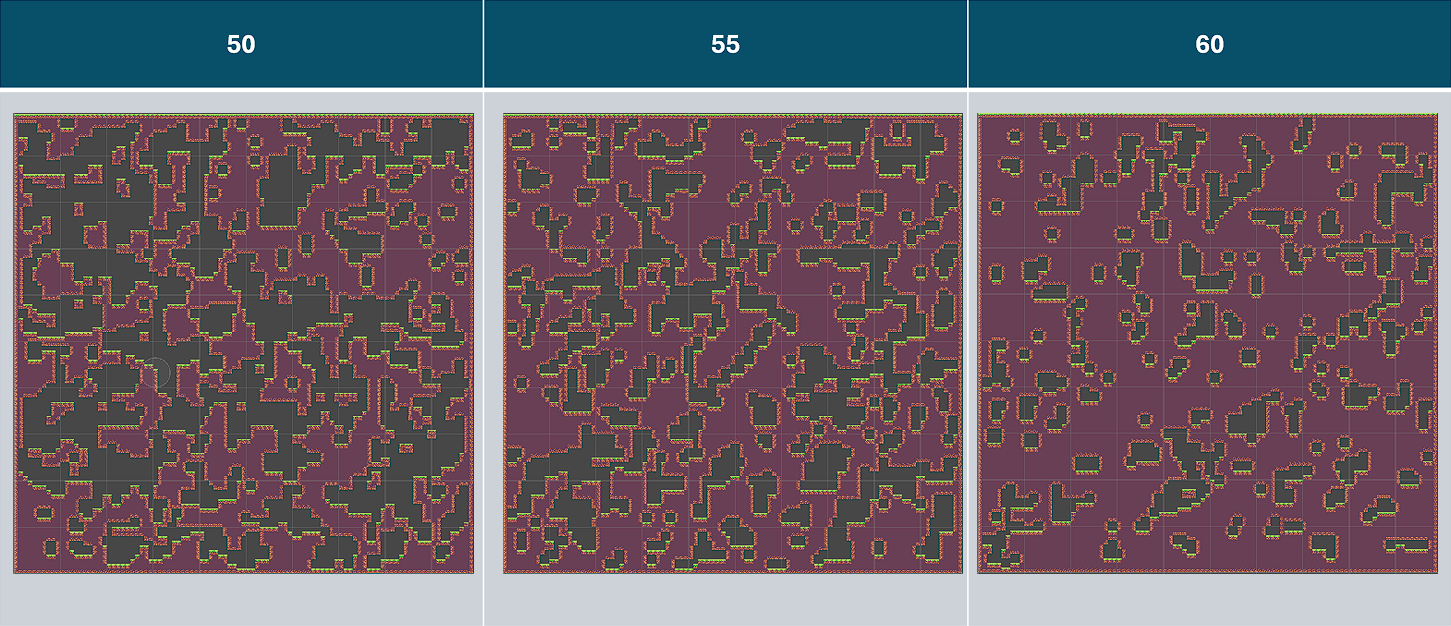
\includegraphics[width=\textwidth]{images/fixedsmoothcellular.png}
\caption{Fixált \texttt{smoothIterations} értékkel és változó \texttt{requiredFloorPercent} értékkel generált térképek}
\label{fig:fixedSmoothCellular}
\end{figure}

\newpage
A fentebb lévő ábrán látható térképeknél a \texttt{smoothIterations} értéke fixen 20, a \texttt{requiredFloorPercent} értéke pedig 50, 55 és 60. Itt már sokkal nagyobb a különbség a legenerált térképek között, minél nagyobb a \texttt{requiredFloorPercent} értéke, annál több olyan cella lesz, amelynek az értéke 1, azaz sokkal sűrűbb lesz a térképünk.

A gond ezzel a procedurális mapgeneráló algoritmussal is az, hogy nem lehet garantálni, hogy olyan térképeket generáljunk, amelyben nincsenek olyan részek, amelyek teljesen elzártak. Ezt az algoritmust inkább 3D-s, Minecraft szerű játékokban tudnám elképzelni, ahol mondjuk az értékes tárgyak elhelyezkedését lehetne meghatározni vele a föld alatt.

\Section{A Random Walk algoritmus (Véletlen bolyongás)}

A véletlen bolyongás algoritmus egy viszonylag egyszerű, de hatékony módszer a procedurális térképgenerálásra, különösen alkalmas kétdimenziós rácsalapú térképekhez. Közismert arról, hogy természetesnek tűnő alakzatokat hoz létre, és összetettebb procedurális generáló rendszerek első lépéseként szolgálhat. Kétdimenziós rácshálózattal összefüggésben a véletlen bolyongást néha „részeges sétának” (Drunkard’s walk-nak) is nevezik, és az elnevezés magától értetődő, ha figyelembe vesszük a működését:\cite{randomwalk}
\begin{enumerate}
\item Hozzunk létre egy $N \times $M méretű rácshálózatot.
\item Válasszunk egy véletlenszerű kezdő pozíciót a rácshálón.
\item Állítsuk be a pozíciót „visited”-re. (Azaz látogatottra.)
\item Válasszunk egy új véletlenszerű pozíciót az aktuális pozíciótól egyetlen cella elmozgatásával (balra / fel / jobbra / le).
\item Ha a pozíció amire érkezünk érvényes (a pozíció nem esik a rácshálón kívülre), akkor ezt az új pozíciót állítsuk be az aktuális pozíciónak.
\item Menjünk vissza a 4. ponthoz, és addig ismételjük, amíg a befejezési feltétel teljesül (például az ismétlések száma).
\end{enumerate}

A modellezés alapvetően egy olyan egyed, amely minden egyes időlépésnél kiszámíthatatlanul mozog bármilyen irányba. Az entitás a korábban meglátogatott cellákba is visszamehet, így a korábbi iterációk nem befolyásolják az aktuális iterációkat, ami a véletlen bolyongást sztochasztikus, memória nélküli folyamattá teszi. Sőt mi több, garantálja, hogy a térkép teljesen összefüggő lesz, mivel csak a szomszédos cellák között mozog. Ez az algoritmus ideális a játékok barlangjainak és túlvilágainak létrehozására, mivel képes összefüggő és terjedelmes térképeket létrehozni.\cite{randomwalk} Egy véletlen bolyongás algoritmussal létrehozott összefüggő térkép \aref{fig:randomwalkfigure}. ábrán megtekinthető.

\begin{figure}[ht]
\centering
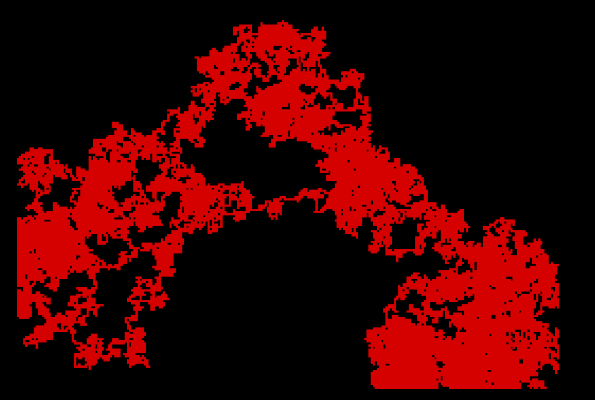
\includegraphics[width =\textwidth]{images/randomwalkfigure.png}
\caption{Egy véletlen bolyongás algoritmussal létrehozott összefüggő térkép \cite{randomwalk}}
\label{fig:randomwalkfigure}
\end{figure}

\newpage
\SubSection{A véletlen bolyongás algoritmus implementálása és vizsgálata}

A \texttt{RandomWalkCave()} metódus a térképrács módosítására szolgál a véletlen bolyongás algoritmuson alapuló procedurális generálási technikával. Ez a függvény egy barlangszerű struktúrát váj ki egy adott kétdimenziós tömbben.

A funkció véletlenszerűen választ ki egy kezdő pozíciót (\texttt{floorX, floorY}) a térkép határain belül, de nem a széleken, hogy biztosítsa, hogy legyen hely a barlang bővítésére. Innen fog kezdődni a véletlen bolyongás. A megadott tartományon belül minden lehetséges kiindulási pozíciónak egyenlő valószínűsége van, hogy kiválasztásra kerüljön, tehát egyenletes eloszlás alapján kerül kiválasztásra a kezdőpozíció.

A \texttt{reqFloorAmount} a térképen lévő összes cellaszám százalékaként kerül kiszámításra. Ez a változó határozza meg, hogy hány cellát kell átalakítani teliből üressé a barlanggenerálás befejezéséhez.

A \texttt{floorCount} nulláról indul, és minden alkalommal növekszik, amikor egy cellát teliből üressé alakítunk.

A \texttt{while} ciklus addig megy, amíg a \texttt{floorCount} értéke el nem éri a \texttt{reqFloorAmount} értékét. A \texttt{while} cikluson belül egy \texttt{switch} utasítást alkalmazok az irányok kezelésére. Az út generálásának a logikája a következő:
\begin{itemize}
\item A switch utasítás minden egyes esete egy iránynak felel meg.
\item Mielőtt az algoritmus bármilyen irányba mozogna, biztosítjuk, hogy a lépés nem halad ki a térkép határain kívülre.
\item 0.eset: Növeljük a \texttt{floorY} értékét, ha a felfelé mozgás a határokon belül marad.
\item 1.eset: Csökkentjük a \texttt{floorY} értékét, ha a lefelé mozgás a határokon belül marad.
\item 2.eset: Növeljük a \texttt{floorX} értékét, ha a jobbra mozgás a határokon belül marad.
\item 3.eset: Csökkentjük a \texttt{floorX} értékét, ha a balra mozgás a határokon belül marad.
\end{itemize}

Minden esetben megnézzük, hogy a jelenlegi pozíció teli-e. Ha az, akkor átkonvertáljuk üresre, és a procedúra addig folytatódik, amíg el nem érjük a kívánt cellák számát. Az alább látható metódus a \cite{mapgenerator} oldal alapján készült.

\begin{java}
public static int[,] RandomWalkCave(
    int[,] map, float seed, int requiredFloorPercent)
{
    //Seed our random
    System.Random rand = new System.Random(
        seed.GetHashCode());

    //Define our start x position
    int floorX = rand.Next(
        1, map.GetUpperBound(0) - 1);
    //Define our start y position
    int floorY = rand.Next(
        1, map.GetUpperBound(1) - 1);
    //Determine our required floorAmount
    int reqFloorAmount = (
        (map.GetUpperBound(1) * map.GetUpperBound(0))
        * requiredFloorPercent) / 100;

    //Used for our while loop,
    //when this reaches our reqFloorAmount
    //we will stop tunneling
    int floorCount = 0;

    //Calculating stepcount and runtime
    int stepCount = 0;
    Stopwatch stopwatch = new Stopwatch();

    //Set our start position
    //to not be a tile (0 = no tile, 1 = tile)
    map[floorX, floorY] = 0;
    //Increase our floor count
    floorCount++;

    stopwatch.Start();
    while (floorCount < reqFloorAmount)
    {
        //Determine our next direction
        int randDir = rand.Next(4);

        stepCount++;
        switch (randDir)
        {
            case 0: //Up
                //Ensure that the edges
                //are still tiles
                if ((floorY + 1) < 
                    map.GetUpperBound(1) - 1)
                {
                    //Move the y up one
                    floorY++;

                    if (map[floorX, floorY] == 1)
                    {
                        //Change it to not a tile
                        map[floorX, floorY] = 0;
                        //Increase floor count
                        floorCount++;
                    }
                }
                break;
            case 1: //Down
                //Ensure that the edges
                //are still tiles
                if ((floorY - 1) > 1)
                {
                    //Move the y down one
                    floorY--;
                    if (map[floorX, floorY] == 1)
                    {
                        //Change it to not a tile
                        map[floorX, floorY] = 0;
                        //Increase the floor count
                        floorCount++;
                    }
                }
                break;
            case 2: //Right
                //Ensure that the edges are still tiles
                if ((floorX + 1) < 
                    map.GetUpperBound(0) - 1)
                {
                    //Move the x to the right
                    floorX++;
                    if (map[floorX, floorY] == 1)
                    {
                        //Change it to not a tile
                        map[floorX, floorY] = 0;
                        //Increase the floor count
                        floorCount++;
                    }
                }
                break;
            case 3: //Left
                //Ensure that the edges are still tiles
                if ((floorX - 1) > 1)
                {
                    //Move the x to the left
                    floorX--;
                    if (map[floorX, floorY] == 1)
                    {
                        //Change it to not a tile
                        map[floorX, floorY] = 0;
                        //Increase the floor count
                        floorCount++;
                    }
                }
                break;
        }
    }
    stopwatch.Stop();
    TimeSpan ts = stopwatch.Elapsed;
    UnityEngine.Debug.Log(
        $"The runtime of the RandomWalkCave() method is " +
        $"{ts.TotalMilliseconds}");
    UnityEngine.Debug.Log(
        $"The stepcount of the RandomWalkCave() method is " +
        $"{stepCount}");
    //Return the updated map
    return map;
}
\end{java}

A továbbiakban a véletlen bolyongás algoritmussal generált térképek vizsgálatával fogok foglalkozni.

Mindegyik generált térkép $100 \times $100-as mátrixnak felel meg, amelyet 1-esekkel töltünk fel. Az első vizsgálat a \texttt{requiredFloorPercent} érték növelésével fog történni. Hat esetet fogok vizsgálni, melyeknél a változó értéke rendre 20, 30, 40, 50, 60 és 70 lesz. A legenerált térképek a megadott \texttt{requiredFloorPercent} értékkel \aref{fig:lowpercentrandomwalk}. ábrán és \aref{fig:highpercentrandomwalk}. ábrán megtekinthetőek.

\begin{figure}[ht]
\centering
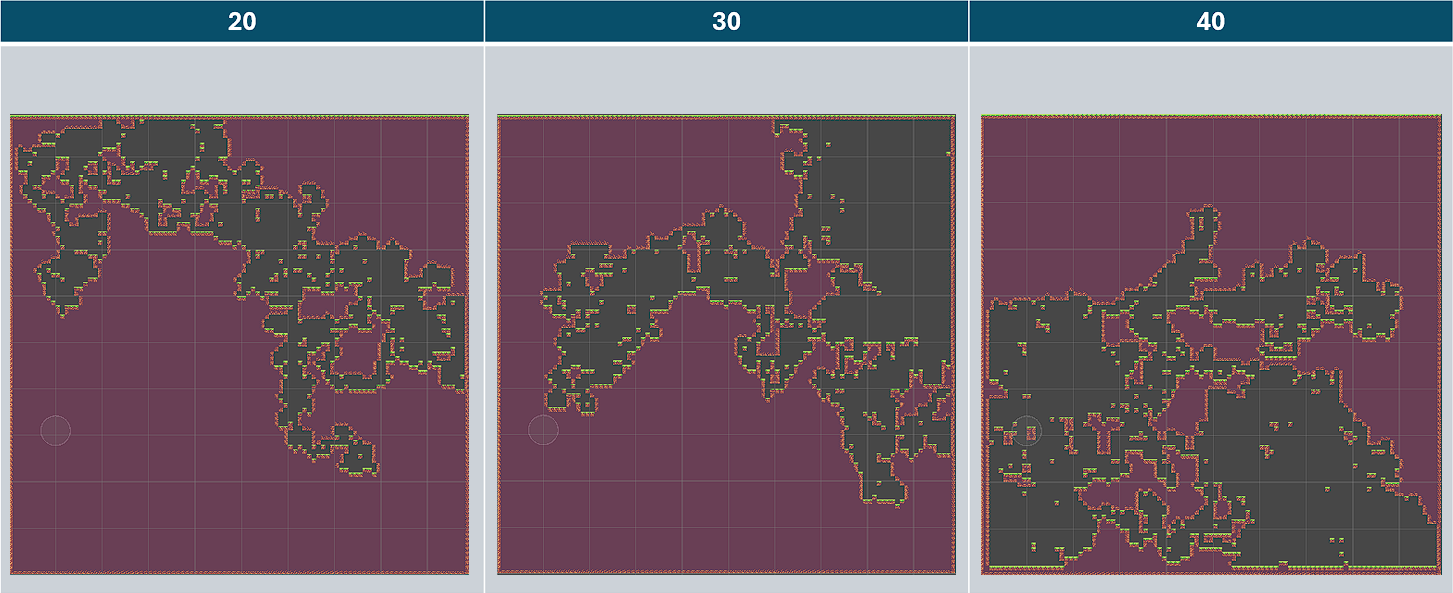
\includegraphics[width = \textwidth]{images/lowpercentrandomwalk.png}
\caption{Azok a térképek, amelye 20, 30 és 40 \texttt{requiredFloorPercent} értékkel lettek generálva}
\label{fig:lowpercentrandomwalk}
\end{figure}

\begin{figure}[ht]
\centering
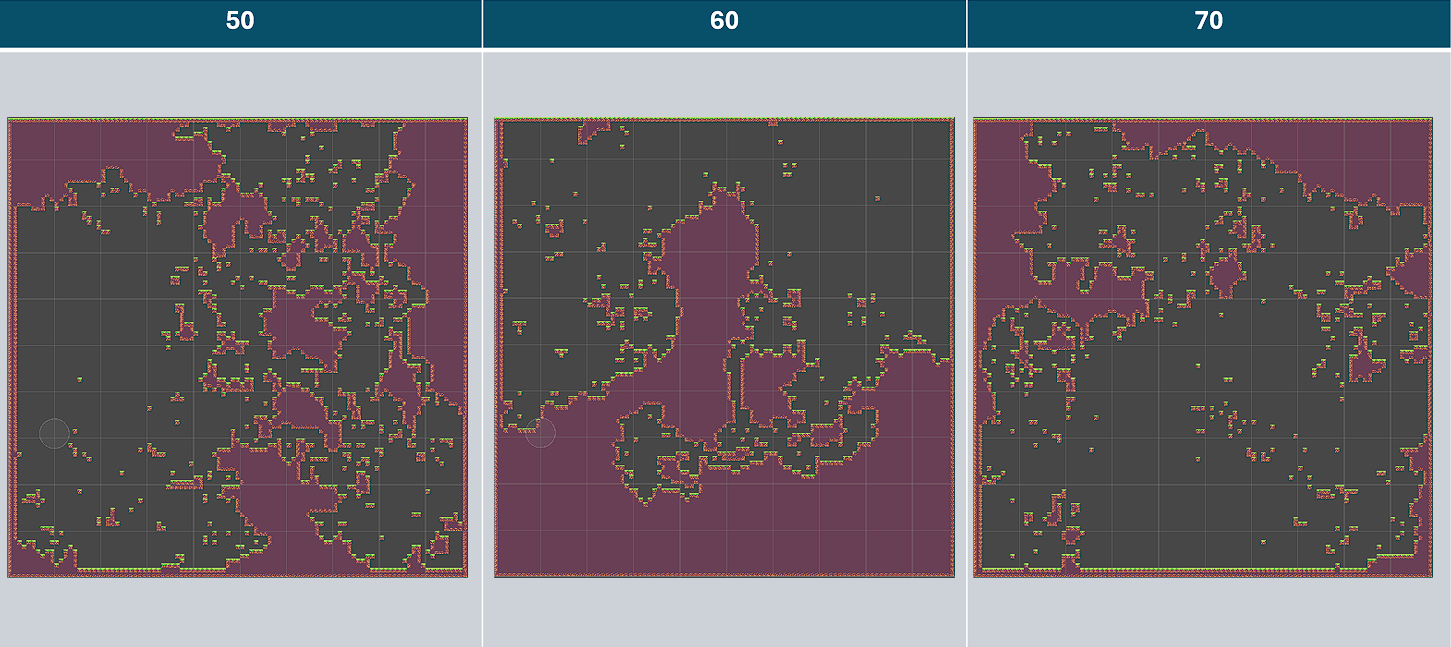
\includegraphics[width = \textwidth]{images/highpercentrandomwalk.png}
\caption{Azok a térképek, amelye 50, 60 és 70 \texttt{requiredFloorPercent} értékkel lettek generálva}
\label{fig:highpercentrandomwalk}
\end{figure}

\newpage
Ahogy az ábrákon is láthatjuk, minél nagyobb a \texttt{requiredFloorPercent} változó értéke, annál több alagutat váj ki magának az algoritmus, azaz annál több olyan cella keletkezik, melynek az értéke 0. Azt is észrevehetjük, hogy nem keletkezik olyan rész a térképen, amely el lenne zárva, azaz teljesen összefüggő mapot kapunk minden egyes esetben.

Minél nagyobb a \texttt{requiredFloorPercent} értéke, annál nagyobb lesz a lépésszáma az algoritmusnak, valamint a futási ideje is nőni fog. Volt néhány olyan eset, ahol nagyobb \texttt{requiredFloorPercent} értéknél kevesebb futási idő, valamint lépésszám volt, de ez elenyésző mennyiségű esetben fordult elő. A lépésszám és a \texttt{requiredFloorPercent} korrelációja \aref{fig:randomwalkgrafikon}. ábrán megtekinthető.

\begin{figure}[ht]
\centering
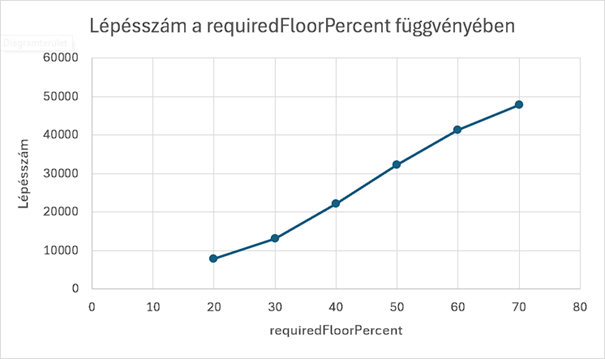
\includegraphics[width = \textwidth]{images/grafikon.png}
\caption{A lépésszám és a requiredFloorPercent kapcsolata}
\label{fig:randomwalkgrafikon}
\end{figure}

\newpage
A következő vizsgálat során változó méretű térképeket fogok generálni, viszont a \texttt{requiredFloorPercent} értékét 45-re fogom fixálni. Ezen térképek legenárálásának szintén a lépésszámát, valamint az idejét fogom vizsgálni. A térképek rendre $30 \times $30, $40 \times $40 és $50 \times $50 méretűek lesznek. A legenerált térképek \aref{fig:changingmaprandomwalk}. ábrán láthatóak.

\begin{figure}[ht]
\centering
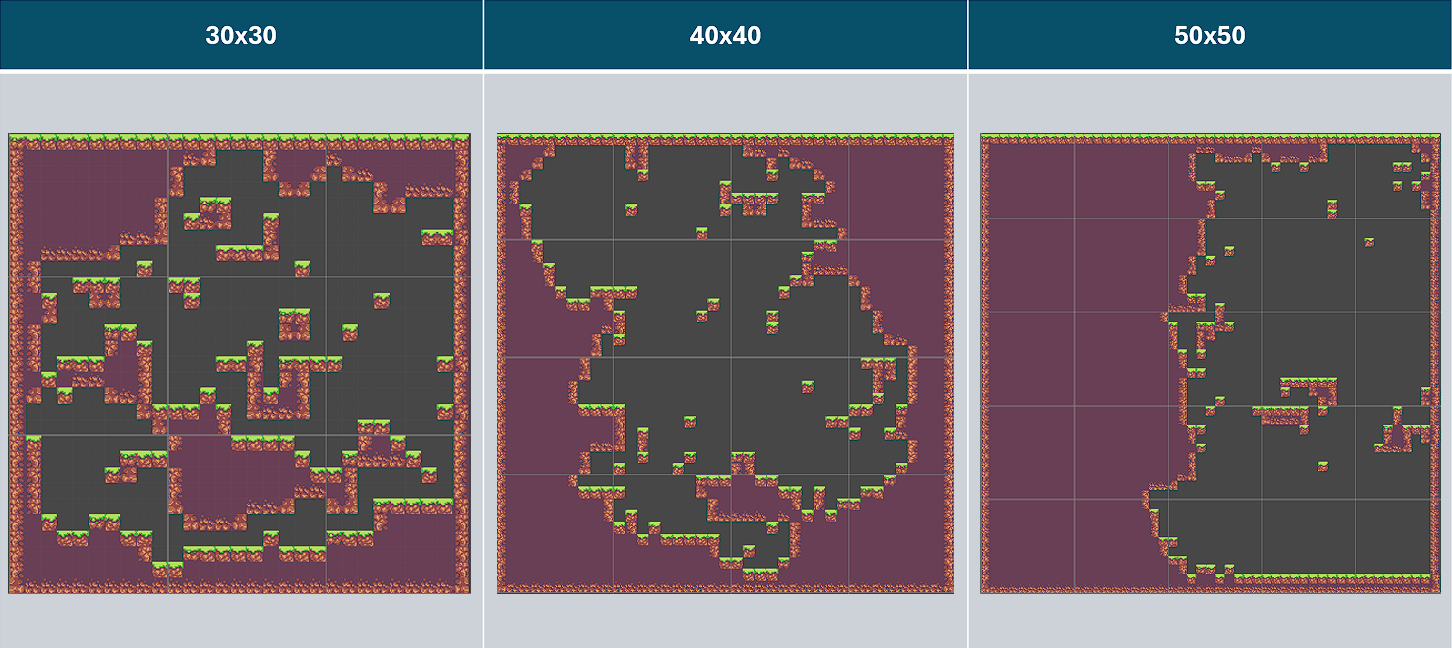
\includegraphics[width = \textwidth]{images/changingmaprandomwalk.png}
\caption{Fixált \texttt{requiredFloorPercent} értékkel, de változó térképmérettel generált mapok}
\label{fig:changingmaprandomwalk}
\end{figure}

A generáláshoz szükséges futási idő, valamint a lépésszám \aref{fig:runtimestepcount1}. ábrán látható.

\begin{figure}[ht]
\centering
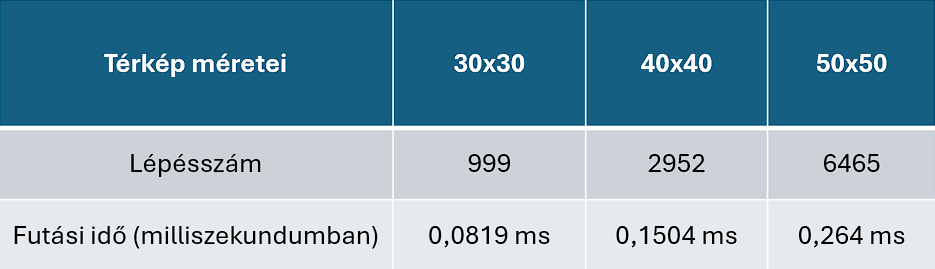
\includegraphics[width=\textwidth]{images/runtime4changinmapsizerandomwalk.png}
\caption{A fixált \texttt{requiredFloorPercent} értékkel és változó térképmérettel rendelkező mapok generálásának lépésszáma és futási ideje}
\label{fig:runtimestepcount1}
\end{figure}

\newpage
További vizsgálatokat fogok az algoritmuson elvégezni, mivel jelenleg egyenletes eloszlást használ az algoritmus, ahol minden fő iránynak (felfelé, lefelé, balra és jobbra) egyenlő a valószínűsége, amely 0,25. Ez egy torzítatlan sétát eredményez, amely egyik irányt sem részesíti előnyben a többivel szemben. Az egyes irányok valószínűségeinek megváltoztatásával különböző hatásokat és mintákat hozhatunk létre a térképgenerálás során.

Az egyik ilyen vizsgálat során nagyobb valószínűséget fogok rendelni az előző lépéssel megegyező irányba történő előrehaladáshoz és kisebb valószínűséget az irányváltoztatáshoz. Ehhez módosítanom kell az egyes lépések kiválasztásának a logikáját.

Először is egy olyan metódust kell implementálni, amely egy nem egyenletes eloszlás alapján választ irányt, majd az egyszerű \texttt{rand.Next(4)} parancsot lecserélni erre a metódusra. A metódusnak a neve a \texttt{ChooseDirectionBias()}.

\begin{java}
private static int ChooseDirectionBias(
    System.Random rand, int[] directions, int lastDirection)
{
    double[] probabilities = 
        new double[directions.Length];

    // 70 percent chance to continue in the same direction
    double bias = 0.7; 

    for (int i = 0; i < directions.Length; i++)
    {
        probabilities[i] = 
            (lastDirection == directions[i]) ? 
            bias : (1 - bias) / (directions.Length - 1);
    }

    double roll = rand.NextDouble();
    double cumulative = 0.0;

    for (int i = 0; i < probabilities.Length; i++)
    {
        cumulative += probabilities[i];
        if (roll < cumulative)
        {
            return directions[i];
        }
    }

    // Fallback
    return directions[directions.Length - 1]; 
}
\end{java}

Az első lépés a valószínűségi tömb inicializálása, amely lebegőpontos számokat fog tartalmazni, és a hossza megegyezik a directions tömb hosszával. Ez a tömb tárolja az egyes irányok valószínűségét. Ezután inicializálunk egy \texttt{bias} nevű változót, amelynek a változtatásával kontrollálhatjuk, hogy mennyire legyen hajlamos az algoritmus ugyanabba az irányba haladni. Az első \texttt{for} cikluson belül számítjuk ki az úgynevezett „elfogult” valószínűséget (biased probability). Ha egy irány megegyezik a \texttt{lastDirection} irányával, akkor nagyobb valószínűséget kap (bias paraméter, jelenleg 70\%-ra állítva). Az összes többi irány egyenlő arányban részesül a fennmaradó 30\%-os valószínűségből.

A következő lépés a random választásnak az implementálása. A \texttt{rand.NextDouble()} parancs egy véletlenszerű lebegőpontos számot generál 0 és 1 között, amely tulajdonképpen egy „roll”-ként működik, hogy eldöntse, melyik irány lesz választva. A második \texttt{for} cikluson a probabilities tömbön iterálunk végig, és kiszámítjuk a kumulatív valószínűséget. Ezután az irányok kiválasztása következik annak ellenőrzésével, hogy a véletlenszerű „roll” az egyes irányok együttes valószínűségi tartományába esik-e. Az első olyan irány lesz kiválasztva, ahol a kumulatív valószínűség meghaladja a „roll” értékét.

A metódus \texttt{return} értékként visszaadja a kiválasztott irányt az eredeti irányok tömbjének megfelelő indexeként.

A továbbiakban a \texttt{ChooseDirectionBias()} metódus beépítésével generált térképeket fogom vizsgálni rögzített $N \times $N méretű pályákon, majd változó méretű pályákon és ezek legenerálásának a futási idejét, valamint lépésszámát is vizsgálni fogom. A vizsgálat során a \texttt{bias} változó értékét fogom módosítani a rögzített $N \times $N  méretű pályákon. A \texttt{requiredFloorPercent} értéke rögzítve lesz, a 45-ös értéken.

Mindegyik generált térkép $100 \times $100-as mátrixnak felel meg, amelyet 1-esekkel töltünk fel. Három esetet fogok vizsgálni, ahol a \texttt{bias} változó értékét fogom módosítani. A \texttt{bias} paraméter értéke rendre 0.6, 0.7 és 0.8 lesz. A generált térképek \aref{fig:fixedPercentRandomWalk}. ábrán láthatóak.

\begin{figure}[ht]
\centering
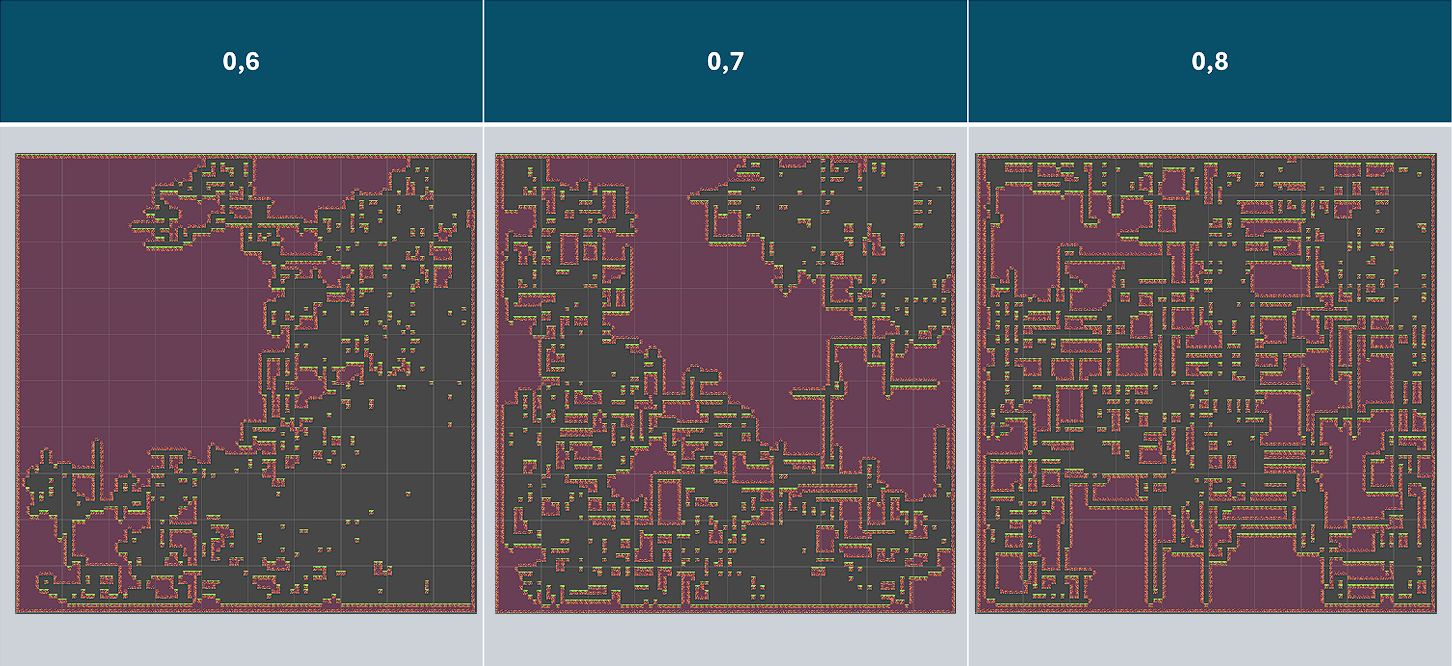
\includegraphics[width = \textwidth]{images/fixedpercentrandomwalk.png}
\caption{Változó \texttt{bias} paraméterekkel generált térképek}
\label{fig:fixedPercentRandomWalk}
\end{figure}

\newpage
Az ábráról, amely a generált térképeket különböző \texttt{bias} értékekkel szemlélteti, miközben a \texttt{requiredFloorPercent} és a térkép mérete állandó, több következtetést is levonhatunk a \texttt{bias} paraméter értékének változtatásának hatásáról.

\textbf{A bias érték hatása:}
\begin{itemize}
\item \textbf{0.6-os érték}: Ezzel az értékkel a pályák kevesebb egyenes vonallal rendelkeznek, egy olyasmi térképet hoz létre, amely kevesebb falat és egy nagy nyitott területet tartalmaz.
\item \textbf{0.7-es érték}: A \texttt{bias} érték növelésével összefüggőbb mintázat kezd kialakulni, az ösvények több és egyenesebb kapcsolatokat kezdenek kialakítani a területek között.
\item \textbf{0.8-as érték}: Ezen a szinten a térkép sok egyenes útvonalat mutat, több kisebb nyitott területtel, amelyeket ezek a kiterjedtebb útvonalak kötnek össze.
\end{itemize}

A térképek generálásának lépésszáma, valamint futási ideje \aref{fig:fixedpercentruntimestepcount}. ábrán látható.

\begin{figure}[ht]
\centering
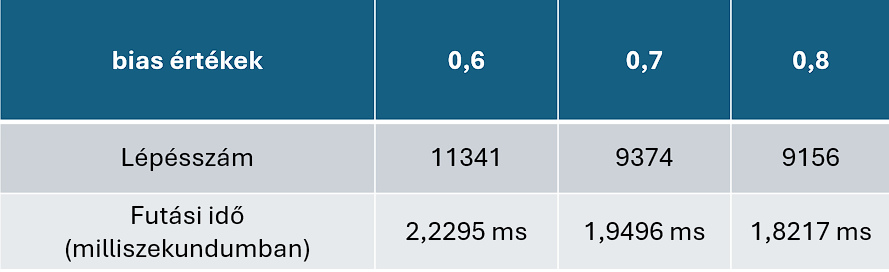
\includegraphics[width=\textwidth]{images/fixedpercentruntimestepcount.png}
\caption{A változó bias értékkel legenerált térképek lépésszáma és futási ideje}
\label{fig:fixedpercentruntimestepcount}
\end{figure}

Mint láthatjuk, alacsonyabb \texttt{bias} érték esetén az algoritmus gyakrabban változtatja az irányt, ami több elfordulást eredményez. Ez összetettebb útvonalakat hoz létre, amelyek általában további lépéseket igényelnek ahhoz, hogy elérjék a térkép szükséges alapszázalékát, mivel az útvonal megfordulhat önmagában, vagy kevésbé közvetlen útvonalon haladhat.

A továbbiakban a változó méretű térképek generálásának a vizsgálatával fogok foglalkozni. Szintén megvizsgálom a futási időt, valamint a lépésszámot. A térképek mérete rendre $50 \times $50, $60 \times $60 és $70 \times $70 méretűek lesznek, a \texttt{bias} változó értékét, valamint a \texttt{requiredFloorPercent} értékét is állandóra állítom. A \texttt{bias} értéke 0.7, a \texttt{requiredFloorPercent} értéke pedig 45 lesz. Az ily módon generált térképek \aref{fig:fixedbiaschangingmapsize}. ábrán, a hozzájuk tartozó lépésszám, valamint futási idő \aref{fig:fixedbiaschangingmapsizeruntimestepcount}. ábrán látható.

\begin{figure}[ht]
\centering
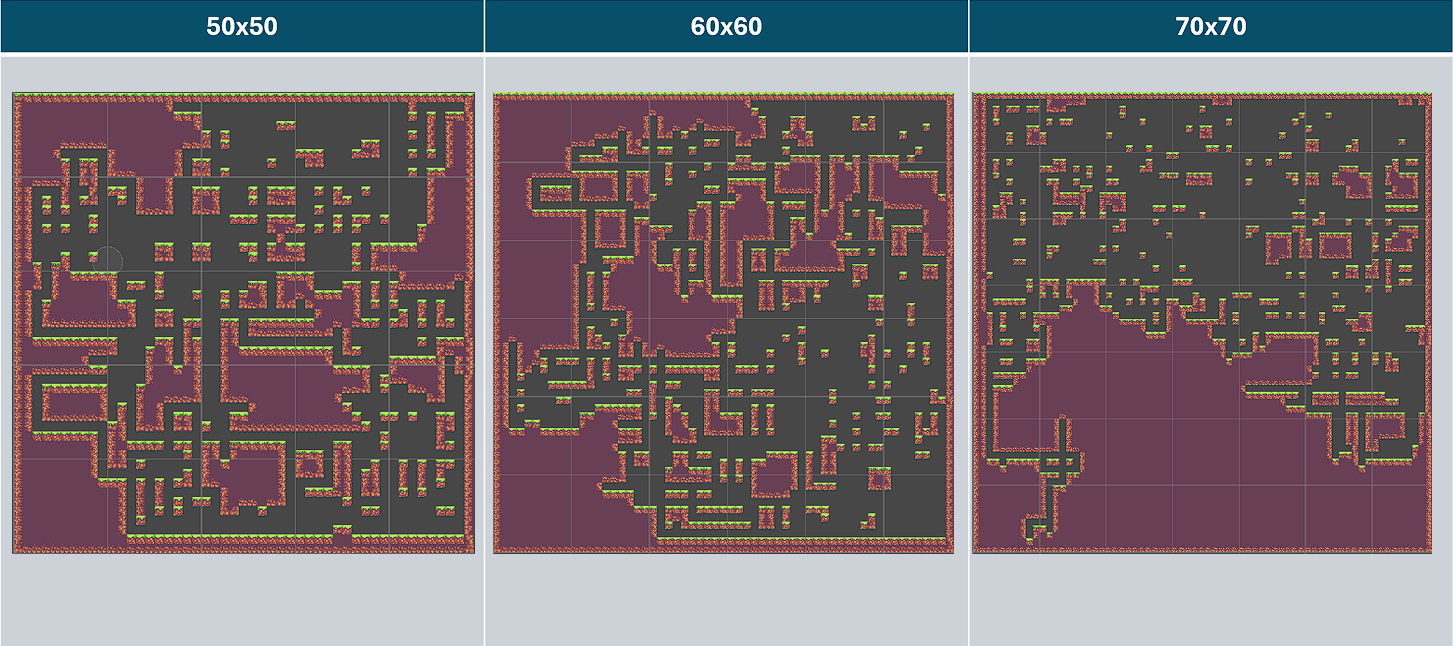
\includegraphics[width=\textwidth]{images/fixedbiaschangingmapsize.png}
\caption{Különböző méretű térképek legenerálása állandó \texttt{bias} értékkel}
\label{fig:fixedbiaschangingmapsize}
\end{figure}

\begin{figure}[ht]
\centering
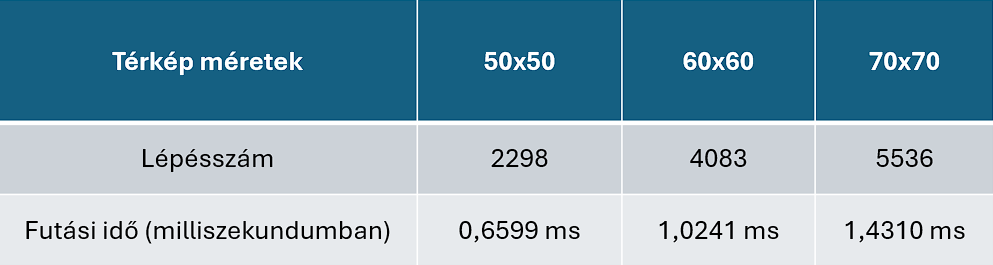
\includegraphics[width=\textwidth]{images/fixedbiaschangingmapsizestepcountruntime.png}
\caption{A különböző méretű térképek generálásához szükséges lépésszám, valamint futási idő}
\label{fig:fixedbiaschangingmapsizeruntimestepcount}
\end{figure}

\newpage
Ahogy az várható volt, minél nagyobb a térkép területe, annál több lépésszám szükséges a kívánt \texttt{requiredFloorPercent} értékének eléréséhez, valamint a futás idő is több lesz.

Úgy vélem, ez az algoritmus felelt meg leginkább az általam felállított követelményeknek, hiszen mindig olyan pályákat generál, amely összefüggő, a térkép szélei mindig falak, így a játékos szabadon navigálhat anélkül, hogy törődnie kellene a leeséssel, nincsenek olyan részek, ahová a játékos ne tudna eljutni, hiszen nincsenek elzárt terek. Ahhoz viszont, hogy a játékos eljusson mindenhová, egy bizonyos játékmechanikát fogok bevezetni, ami nem más mint, a grappling hook.


